\documentclass{article}[12pt]
\renewcommand{\baselinestretch}{1.5}
\setlength{\parskip}{1em}

\usepackage[parfill]{parskip}
\usepackage[affil-it]{authblk}
\usepackage[space]{grffile}

\usepackage[a4paper]{geometry}
\geometry{verbose}
\usepackage{float}
\usepackage{graphicx}
\graphicspath{{figures/}}
\usepackage{setspace}
\usepackage{caption}

\usepackage[utf8]{inputenc}
\usepackage[english]{babel}

\usepackage{latexsym,textcomp,longtable,tabulary}
\usepackage{booktabs,array,multirow,braket}
\usepackage{amsfonts,amsmath,amssymb,mathbbol,calc}
\usepackage{subfigure,color,blindtext,enumitem,siunitx}
\usepackage[colorinlistoftodos]{todonotes}

\usepackage{mathtools}
\usepackage{url,hyperref,etoolbox}
\numberwithin{equation}{section}
\hypersetup{colorlinks=false,pdfborder={0 0 0}}

%+figure layout options
\restylefloat{figure}
\setlist{leftmargin=*,before=\setlength{\rightmargin}{\leftmargin}}
%-figure layout options


\providecommand\citet{\cite}
\providecommand\citep{\cite}
\providecommand\citealt{\cite}

\makeatletter
\makeatother

\begin{document}

\title{
Time-series segmentation and latent\\ representation of musical instruments
}

\author{Gregory Szep}
\affil{King's College London}
\date{\today}
\maketitle

\abstract{Music information retrieval tasks serve as faithful benchmarks for
time-series analysis pipelines due to the availability of strongly labelled
training data such as MusicNet. Clustering algorithms in spectral sub-spaces,
hidden Markov models and causal convolutional neural networks are compared in
their ability to transform time-series to a continuous latent space that
clusters eleven orchestral instruments. The latent space is evaluated
quantitatively with precision-recall metrics obtained by comparing the
instrument prediction from a segment of audio to the ground truth obtained
from musical scores, and qualitatively by generating samples of audio for given
regions in the latent space.}
\section{Problem Outline}
\subsection{Mapping time-series to latent space}
The input data are single channel time-series points $\mathcal{D}=\{x(t_1)\dots
x(t_N)\}$ sampled at frequency $f$ from an underlying continuous state-time
process $x(t)$, that is the oscillating sound waves emitted by a live orchestra.

\begin{figure}[H]
\centering{}
\captionsetup{justification=centering}
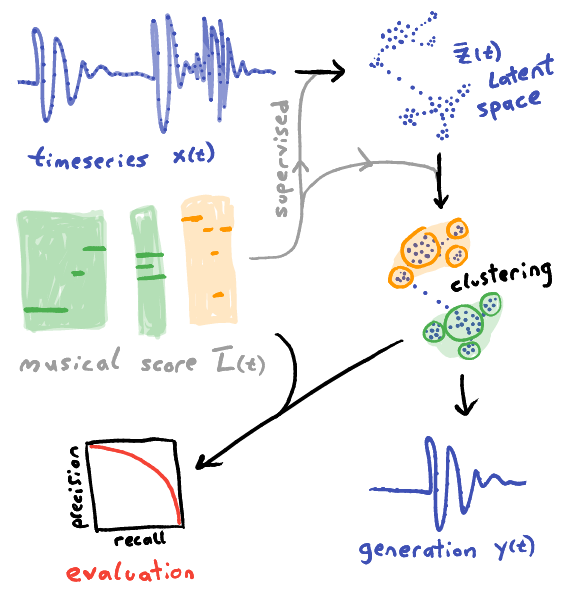
\includegraphics[scale=0.35]{methods}
\label{fig:methods}
\end{figure}

\section{Clustering in spectral sub-spaces} \vspace{-10pt}

\section{Hidden Markov models} \vspace{-10pt}
\section{Causal convolutional networks}
Convolutional architectures have become popular due to their ability to compress spatio-temporal
information for discrimination and generation tasks \cite{Oord2016PixelNetworks,GoodfellowGenerativeNets}.
A causal convolutional network \cite{Oord2016WaveNet:Audio} --- which encodes the arrow of time in
its architecture --- is trained for the audio segmentation task.


\bibliography{mendeley_v2}
\bibliographystyle{ieeetr}
\end{document}
